\begin{frame}
\frametitle{Numerical Simulations for Scientific Discovery}
\framebox{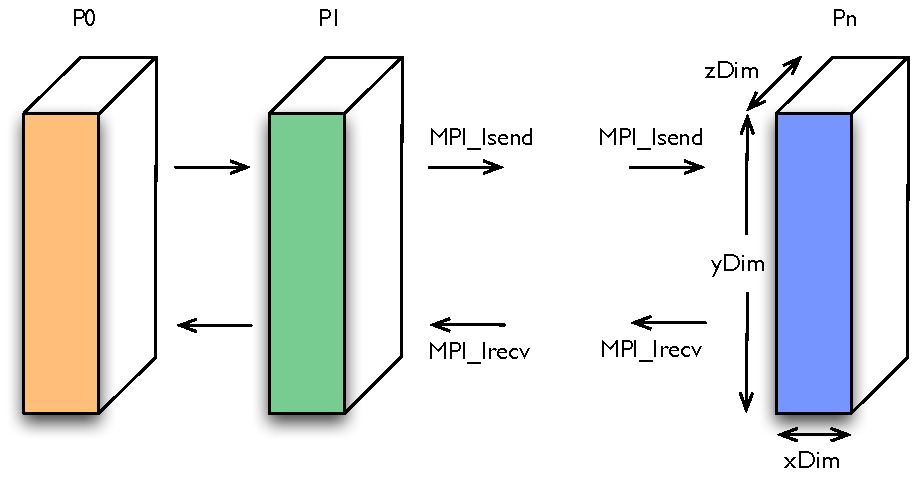
\includegraphics[width=\textwidth]{images/mpi_decomp}}
\begin{center}
Model bulk-synchronous Numerical Simulation
\end{center}
\end{frame}

\begin{frame}[Core Problem for Bulk-synchronous Simulations]
\frametitle{Introduction}
\begin{itemize}
\item \small In 2009, Noise Amplification Problem was shown
  fundamental inhibitor for bulk-synchronous MPI applications running
  at full-scale (at 1 mill. nodes) on a supercomputer simulator.
\item \small Leaves a big question for how to cost-effectively do
  numerical simulations on future supercomputers.
\item \small We have a solution: use within-node resilient scheduling
  ($\mu$-scheduling).
\item \small Can use our techniques in your application codes to
  reduce costs of running full-scale simulations.
\end{itemize}
\end{frame}

\begin{frame}
\frametitle{Core Strategy of our runtime software}
\framebox{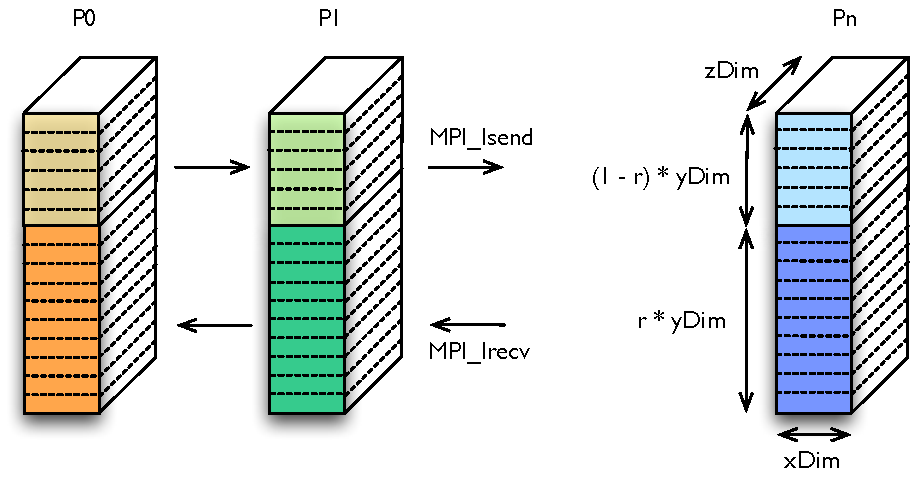
\includegraphics[width=\textwidth]{images/hybrid_decomp}}
\begin{center}
Model numerical simulations with our $\mu$-scheduling runtime software integrated.
\end{center}
\end{frame}

%\begin{frame}
%\frametitle{Evidence of problem on current machines}
%\begin{itemize}
%\item NAP causes 28\% degradations on Jaguar at full scale.
%\item NAP cause 37\% degradations on Ranger at full scale.
%\item Through simulation of exascale machines, these numbers shoot up to 47\% and 53\% on Jaguar and Ranger respectively.
%\end{itemize}
%\end{frame}

\begin{frame}
\frametitle{Variants of  $\mu$-Scheduling}
\begin{itemize}
\item Variable Tasklet Granularity $\mu$-scheduling: Resilient to variable length noise.
\item Weighted Dynamic $\mu$-scheduling: Resilient to periodic noise.
\item Generalized Slack-conscious $\mu$-scheduling: Per-MPI process resilience, where amplification is different across different MPI processes.
\end{itemize}
\end{frame}

\begin{frame}
\frametitle{Our Results at Scale}
\begin{columns}
  \column{0.5\textwidth}
  \begin{enumerate}
  \item \tiny Slack-conscious $\mu$-scheduling provides largest perf. gains on both machines.
  \item \tiny Variable tasklet $\mu$-scheduling gives moderate perf. gains on machine with variable length noise(Ranger), while having no effect on fixed length noise machine(Jaguar).
  \item \tiny Weighted $\mu$-scheduling provides gives moderate perf. gains on machine with periodic noise(Jaguar), without causing degradation on a machine that only has probabilisic noise (Ranger).
  \item \tiny Overall, we get 45\% perf. gains using all these techniques together.
  \item \tiny Our runtime software applies all of these together for your application.
  \end{enumerate}
  \column{0.5\textwidth}
  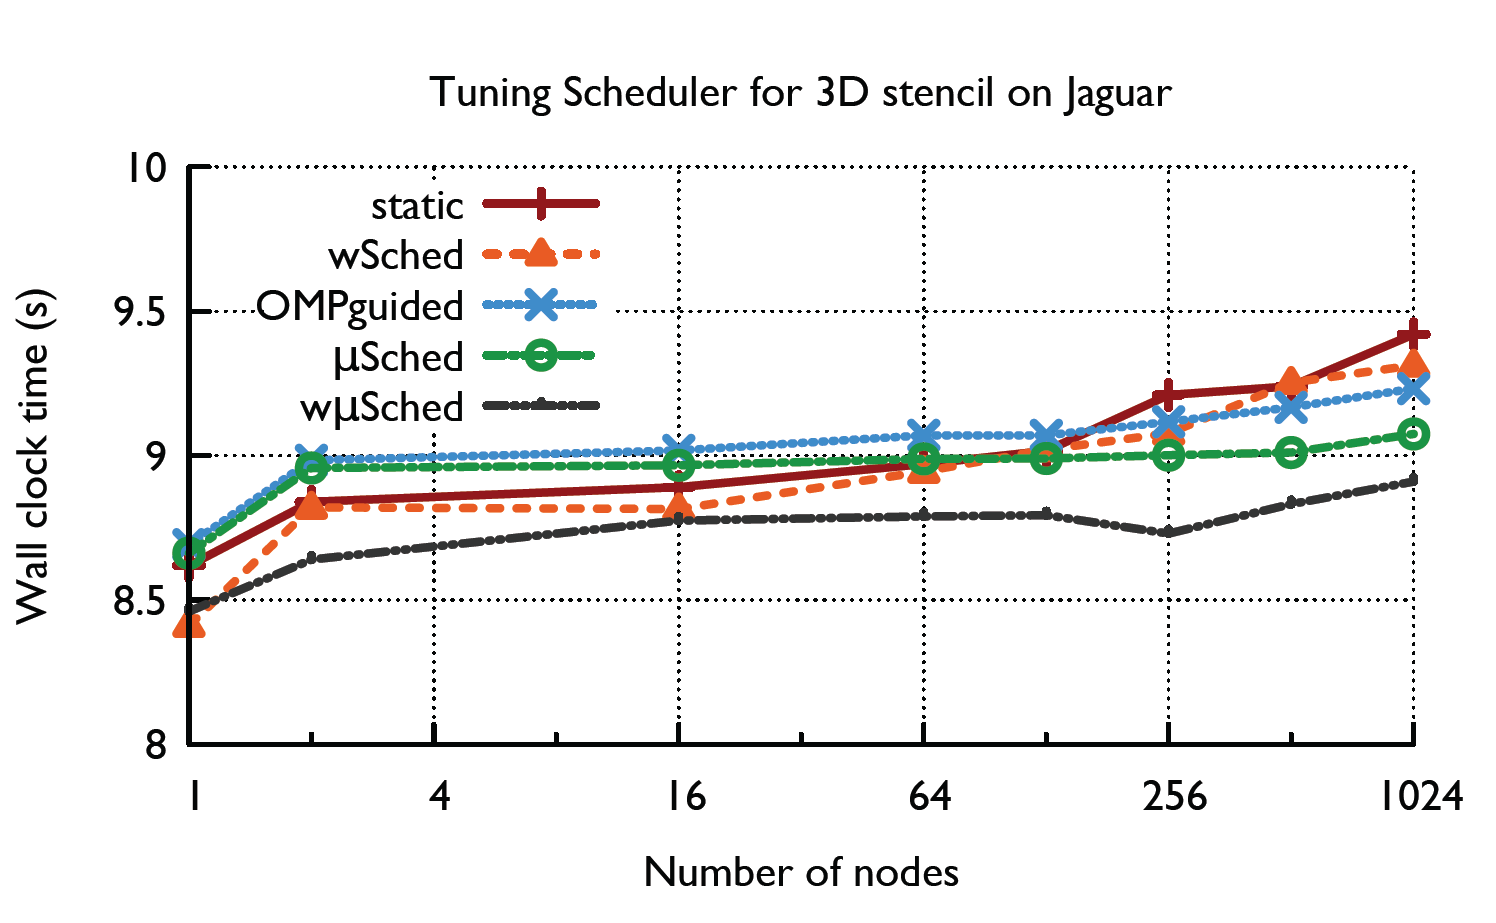
\includegraphics[width=\textwidth]{images/schedulerTuningJaguar} \\
  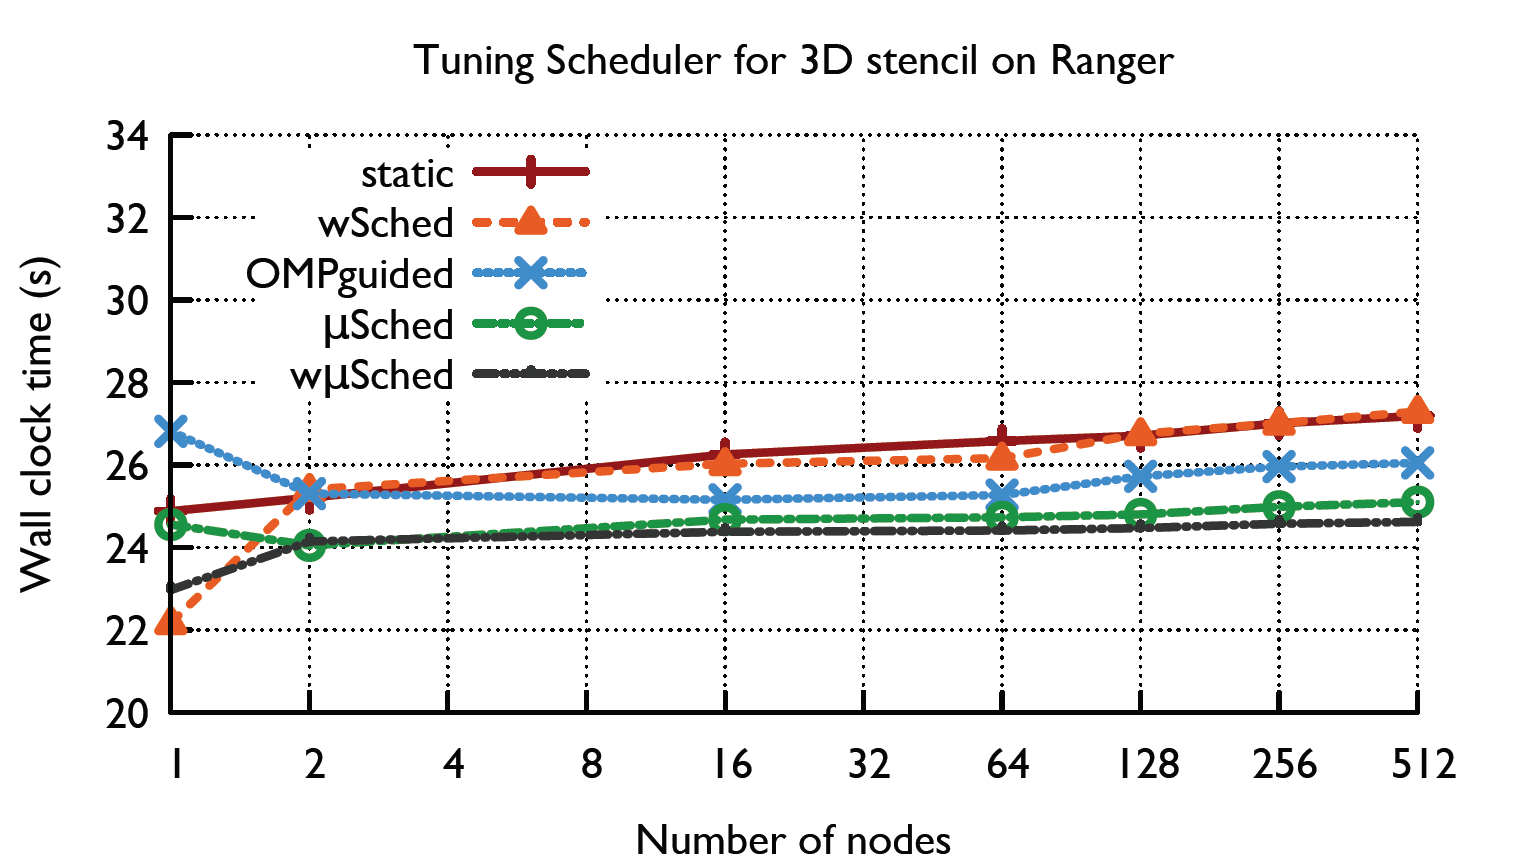
\includegraphics[width=\textwidth]{images/schedulerTuningRanger}
\end{columns}
\end{frame}

\begin{frame}
  \frametitle{Conclusions}
  \begin{itemize}
  \item Several scientific codes are bulk-synchronous in nature, and thus will suffer the noise amplification problem.
  \item We get significant (up to 55\%) performance gains using our techniques,  in the presence of NAP.
  \item Using our techniques, you will be able to \textit{do more science per hour}.
  \item You can obtain our software on the confluence website.  We hope that you will consider it before your next large-scale application run!
  \end{itemize}
\end{frame}
